\documentclass{article}
\usepackage[nonatbib]{project}
\usepackage{watml}
\usepackage[ruled,vlined]{algorithm2e}
\usepackage[normalem]{ulem}
\usepackage{setspace}
% use Times
\usepackage{times}
% For figures
\usepackage{graphicx} % more modern
%\usepackage{epsfig} % less modern
%\usepackage{subfig} 
\usepackage{tikz}
\usetikzlibrary{arrows.meta, calc, positioning}

% path to figure folder
\graphicspath{{../fig/}}
\usepackage{amsmath}
\usepackage{tikz}
\usepackage{pgfplots}
\pgfplotsset{compat=1.17}
% bib file for references
\addbibresource{ref.bib}

\title{Stochastic model-based minimization of weakly convex functions}

\author{
	Fengjing Zhu \\
	Institutes of Science and Development\\
	Chinese Academy of Sciences\\
	Beijing \\
	\texttt{zhufengjing24@mails.ucas.ac.cn} 
}

\begin{document}
\maketitle

\begin{abstract}
This report reviews the paper \textit{Stochastic Model-Based Minimization of Weakly Convex Functions}, which develops a general framework for minimizing weakly convex and possibly nonsmooth functions via stochastic models. The proposed algorithm iteratively samples a stochastic one-sided model of the objective and performs a proximal minimization step. Under standard Lipschitz and weak convexity assumptions, the authors prove that the expected norm of the gradient of the Moreau envelope converges at a rate of $\mathcal{O}(k^{-1/4})$. The framework unifies and establishes complexity guarantees for several key algorithms, including the stochastic proximal point, proximal subgradient, and prox-linear methods. This report summarizes the algorithmic structure, theoretical analysis, and practical implications of the results. For code and reproducibility, see: \href{https://github.com/ina2002/HW.git}{\texttt{link}}.
\end{abstract}


\section{Introduction}

Optimization is fundamental in machine learning, signal processing, and operations research. Many real-world problems, such as robust regression and neural network training, are nonconvex and nonsmooth, making classical optimization techniques inadequate.

A key class of interest is \emph{weakly convex functions}, which allow convexity after adding a quadratic term. To address stochastic minimization under such settings, Davis and Drusvyatskiy propose a unified stochastic model-based framework. This approach replaces exact gradients with one-sided model approximations and introduces regularization via proximal steps.

Their algorithm covers stochastic proximal point, prox-linear, and subgradient methods, and evaluates stationarity via the Moreau envelope. It achieves the first $\mathcal{O}(k^{-1/4})$ convergence guarantee for this broad problem class.

The overall framework is summarized in Figure~\ref{fig:overview}.

\begin{figure}[h]
\centering
\scalebox{0.7}{
  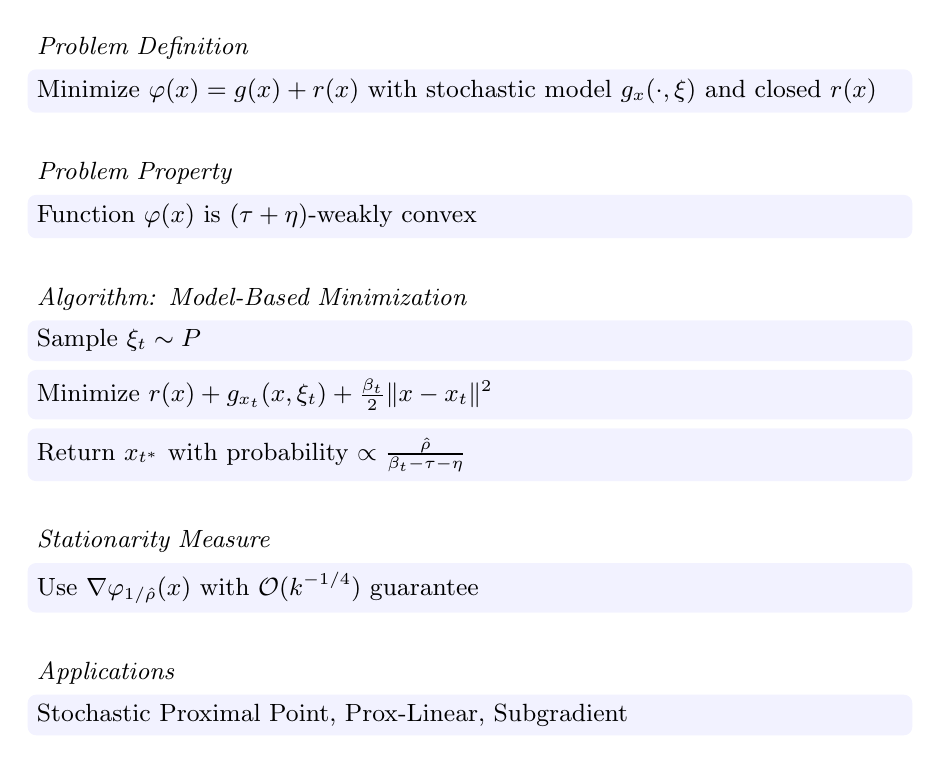
\begin{tikzpicture}[
  font=\small, 
  every node/.style={font=\small},
    box0/.style={
  rectangle, minimum height=0.2cm, minimum width=11cm,
  text width=11cm, align=left, rounded corners=3pt,anchor=west
}, 
  box/.style={
  rectangle, minimum height=0.5cm, minimum width=11cm,
  text width=11cm, align=left, rounded corners=3pt,
  fill=blue!5, anchor=west
}, 
  bendline/.style={draw, thick, -{Stealth}, rounded corners=8pt}
  ]

% Problem Definition
\node[box0] (define0) {\textit{Problem Definition}};
\node[box, below=0cm of define0] (define) {Minimize $\varphi(x) = g(x) + r(x)$ with stochastic model $g_x(\cdot,\xi)$ and closed $r(x)$};

% Problem Property
\node[box0, below=0.5cm  of define] (property0) {\textit{Problem Property}};
\node[box, below=0cm  of property0] (property) {Function $\varphi(x)$ is $(\tau + \eta)$-weakly convex};

% Algorithm
\node[box0, below=0.5cm  of property] (algo0) {\textit{Algorithm: Model-Based Minimization}};
\node[box, below=0cm of algo0] (algo1) {Sample $\xi_t \sim \mathbb{P}$};
\node[box, below=0.1cm of algo1] (algo2) {Minimize $r(x) + g_{x_t}(x,\xi_t) + \frac{\beta_t}{2}\|x - x_t\|^2$};
\node[box, below=0.1cm of algo2] (algo3) {Return $x_{t^*}$ with probability $\propto \frac{\hat{\rho}}{\beta_t - \tau - \eta}$};

% Evaluation
\node[box0, below=0.5cm of algo3] (eval0) {\textit{Stationarity Measure}};
\node[box, below=0cm of eval0] (eval) {Use $\nabla \varphi_{1/\hat{\rho}}(x)$ with $\mathcal{O}(k^{-1/4})$ guarantee};

% Applications
\node[box0, below=0.5cm of eval] (apps0) {\textit{Applications}};
\node[box, below=0cm of apps0] (apps) {Stochastic Proximal Point, Prox-Linear, Subgradient};

\end{tikzpicture}}
\caption{Overview: from problem setup to algorithm, analysis, and applications.}
\label{fig:overview}
\end{figure}



\section{Related Works}

Nonsmooth, nonconvex optimization problems arise in diverse domains such as phase retrieval, covariance estimation, and neural network training. Classical methods often struggle due to non-differentiability and non-convexity. Recent advances—including subgradient methods~\parencite{davis2018subgradient}, proximal algorithms~\parencite{duchi2019solving}, and convex relaxations~\parencite{chen2014exact}—offer partial remedies, but typically depend on structural assumptions or careful initialization.

The \textit{Moreau envelope} plays a central role in analyzing such problems, providing a smooth surrogate whose gradient quantifies stationarity. Davis and Drusvyatskiy leveraged this in a stochastic model-based framework, establishing the first $\mathcal{O}(k^{-1/4})$ convergence rate for weakly convex functions.

Extensions of the envelope to \textit{Bregman distances}~\parencite{kan2012bregman, heinze2022bregman} have broadened its use in variational analysis and imaging~\parencite{durmus2018efficient}, though most results remain limited to convex settings.

In application, \textit{Nonnegative Matrix Factorization (NMF)}~\parencite{gillis2017introduction} exemplifies constrained nonconvex problems, but remains challenging under noise and incomplete observations.


\section{Main Results}

\subsection{Problem Setting}

We consider the stochastic composite optimization problem:
\begin{equation}
\min_{x \in \mathbb{R}^d} \,\, \varphi(x) := g(x) + r(x),
\label{eq:main}
\end{equation}
where \( g: \mathbb{R}^d \to \mathbb{R} \) is possibly nonconvex and nonsmooth, and \( r: \mathbb{R}^d \to \mathbb{R} \cup \{\infty\} \) is a proper closed function, often used for regularization or constraints.

The algorithm accesses \( g \) via a stochastic one-sided model \( g_x(y, \xi) \), where \( \xi \sim \mathbb{P} \). We assume:

\begin{itemize}
    \item[(A1)] i.i.d. samples \( \xi_t \sim \mathbb{P} \) are available;
    \item[(A2)] \( \mathbb{E}_\xi[g_x(x, \xi)] = g(x) \), and 
  \( 
    \mathbb{E}_\xi[g_x(y, \xi)] \ge g(y) - \frac{\tau}{2} \|y - x\|^2;
    \)
    \item[(A3)] \( y \mapsto g_x(y, \xi) + r(y) \) is \( \eta \)-weakly convex;
    \item[(A4)] \( g \) and \( g_x(\cdot, \xi) \) are \( L \)-Lipschitz in expectation.
\end{itemize}

Then \( \varphi \) is \( (\tau + \eta) \)-weakly convex, satisfying:
\[
f(\lambda x + (1 - \lambda)y) \leq \lambda f(x) + (1 - \lambda) f(y) + \frac{\rho \lambda (1 - \lambda)}{2} \|x - y\|^2.
\]

\subsection{Algorithm Description}

The method follows a stochastic model-based minimization framework, where at each step, a model of the objective is sampled and minimized with a proximal term. The procedure is shown in Algorithm~\ref{alg:main}.

\begin{algorithm}[H]
\caption{Stochastic Model Based Minimization}
\label{alg:main}
\KwIn{$x_0 \in \mathbb{R}^d$, parameters $\hat{\rho} > \tau + \eta$, sequence $\{\beta_t\}_{t=0}^T \subset (\hat{\rho}, \infty)$, iteration count $T$}

\For{$t = 0$ \KwTo $T$}{
  Sample $\xi_t \sim \mathbb{P}$\;
  Set $x_{t+1} = \arg\min\limits_{x} \big\{ r(x) + g_{x_t}(x, \xi_t) + \frac{\beta_t}{2} \|x - x_t\|^2 \big\}$\;
}
Sample $t^* \in \{0, \ldots, T\}$ with probability $\mathbb{P}(t^* = t) \propto \frac{\hat{\rho} - \tau - \eta}{\beta_t - \eta}$\;
\KwOut{$x_{t^*}$}
\end{algorithm}

\subsection{Stationarity Measure via Moreau Envelope}

To evaluate convergence, we use the \textit{Moreau envelope}:
\[
\varphi_\lambda(x) := \inf_{y} \left\{ \varphi(y) + \frac{1}{2\lambda} \|y - x\|^2 \right\},
\]
which is differentiable if $\varphi$ is $\rho$-weakly convex and $\lambda < 1/\rho$. Its gradient,
\[
\nabla \varphi_\lambda(x) = \frac{1}{\lambda}(x - \text{prox}_{\lambda \varphi}(x)),
\]
serves as a continuous stationarity measure.

\textbf{Main Result.} Under (A1)–(A4), the output $x_{t^*}$ satisfies:
\begin{equation}
\mathbb{E}\left[ \|\nabla \varphi_{1/\hat{\rho}}(x_{t^*})\|^2 \right]
\leq
\frac{ \hat{\rho} (\varphi_{1/\hat{\rho}}(x_0) - \min \varphi) + 2\hat{\rho}^2 L^2 \sum_{t=0}^T \frac{1}{(\beta_t - \eta)(\beta_t - \hat{\rho})} }{ \sum_{t=0}^T \frac{2(\hat{\rho} - \tau - \eta)}{\beta_t - \eta} }.
\label{eq:moreau_rate}
\end{equation}

\textbf{Convergence Rate.} Choosing $\beta_t = \hat{\rho} + \frac{1}{\alpha\sqrt{T+1}}$ yields
\[
\mathbb{E}\left[ \|\nabla \varphi_{1/\hat{\rho}}(x_{t^*})\|^2 \right] = \mathcal{O}(T^{-1/2}),
\]
implying complexity $\mathcal{O}(\varepsilon^{-2})$ for $\varepsilon$-stationarity.

\textbf{Proof Sketch.} The proof applies Lemma~3.1 to bound the envelope value at $x_{t+1}$:
\[
\mathbb{E}_t[\varphi_{1/\hat{\rho}}(x_{t+1})] \leq \varphi_{1/\hat{\rho}}(x_t) - \frac{\hat{\rho}(\hat{\rho} - \tau - \eta)}{2(\beta_t - \eta)} \|x_t - \hat{x}_t\|^2 + \frac{2\hat{\rho}^2 L^2}{(\beta_t - \eta)(\beta_t - \hat{\rho})}.
\]
Summing over $t$ and using $\varphi_{1/\hat{\rho}}(x_{t+1}) \geq \min \varphi$ leads to:
\[
\mathbb{E} \left[ \sum_{t=0}^{T} \frac{\hat{\rho} - \tau - \eta}{\beta_t - \eta} \|x_t - \hat{x}_t\|^2 \right]
\leq
2 \cdot \frac{\varphi_{1/\hat{\rho}}(x_0) - \min \varphi}{\hat{\rho}} + 4L^2 \sum_{t=0}^{T} \frac{1}{(\beta_t - \eta)(\beta_t - \hat{\rho})}.
\]
Since $\nabla \varphi_{1/\hat{\rho}}(x_t) = \hat{\rho}(x_t - \hat{x}_t)$, we obtain the final bound.

\subsection{Special Cases}

The framework recovers several classical methods by varying model type and assumptions, summarized in Table~\ref{tab:special_cases}.

\begin{table}[h]
\centering
\caption{Special Cases under the General Framework}
\label{tab:special_cases}
\begin{tabular}{lll}
\toprule
Method & Model Type & Key Assumptions \\
\midrule
\textit{Stochastic Proximal Point} & Exact & $\tau = 0$, $\eta = \rho$ \\
\textit{Proximal Subgradient} & Linear & Bounded variance \\
\textit{Prox-Linear} & Composite   & Smooth $c$, convex $h$ \\
\bottomrule
\end{tabular}
\end{table}

\subsection{Numerical Experiment}

We consider the stochastic logistic regression problem:
\[
\min_{x \in \mathbb{R}^d} \varphi(x) := g(x) + r(x),
\]
where \(g(x) = \mathbb{E}_\xi \left[ \log \left( 1 + \exp(-y z^\top x) \right) \right]\) with \(\xi = (z, y)\), \(y \in \{-1, 1\}\), and \(r(x) = \frac{\lambda}{2} \|x\|^2\) with \(\lambda = 0.1\).

We initialize at \(x_0 = 0\) and run for \(T = 100\) iterations, setting
\(
\tau + \eta = 2, \quad \hat{\rho} = 3, \quad \beta_t > \hat{\rho}.
\)

The experiment is repeated 5 times to evaluate robustness. Results are shown in Figure~\ref{fig:moreau_gradient} and~\ref{fig:final_loss}.

\begin{figure}[h]
\centering
\begin{minipage}{0.55\textwidth}
\centering
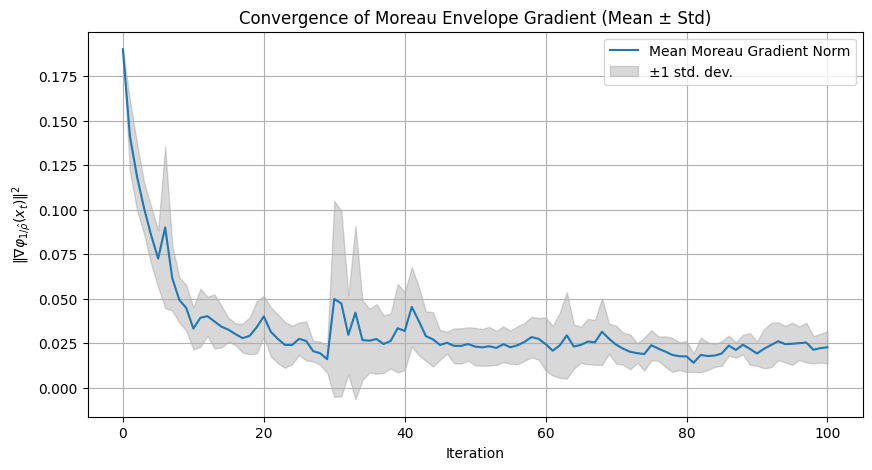
\includegraphics[width=\textwidth]{moreau_gradient_convergence.png}
\caption{Convergence of Moreau Envelope Gradient}
\label{fig:moreau_gradient}
\end{minipage}
\hfill
\begin{minipage}{0.35\textwidth}
\centering
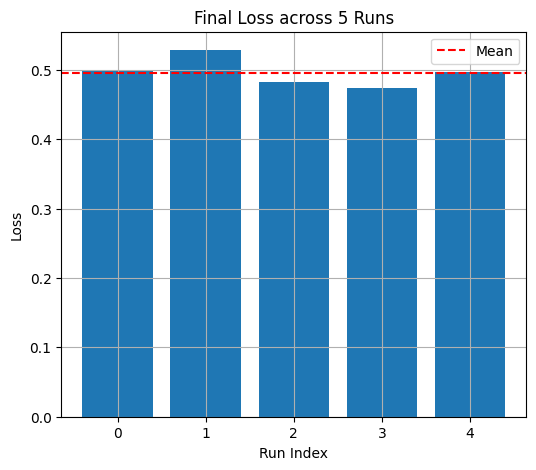
\includegraphics[width=\textwidth]{final_loss_comparison.png}
\caption{Final Loss across 5 Runs}
\label{fig:final_loss}
\end{minipage}
\end{figure}

 

\section{Conclusion}

This report examined the stochastic model-based minimization framework for weakly convex functions proposed by Davis and Drusvyatskiy. Its main contribution is a unified algorithmic scheme that generalizes several classical methods and provides the first complexity guarantees for convergence to approximate stationary points. A central analytical tool is the Moreau envelope, whose gradient yields a smooth measure of near-stationarity.

The framework stands out for its generality and minimal assumptions: it requires only stochastic one-sided models accurate in expectation, making it widely applicable. It achieves an $\mathcal{O}(k^{-1/4})$ convergence rate in the Moreau envelope gradient norm, improving known results in certain settings.

However, limitations remain. The theory focuses on first-order stationarity, with second-order or global analysis still unexplored. Performance may be sensitive to hyperparameters such as $\beta_t$ and $\hat{\rho}$, suggesting the value of adaptive tuning. Future enhancements could address heavy-tailed noise, variance reduction, or structured modeling (e.g., Hessian surrogates) to improve robustness.

Promising directions include applications to large-scale nonconvex learning problems—such as deep networks and stochastic reinforcement learning—where this framework's combination of flexibility and theoretical guarantees offers a compelling foundation for stochastic nonsmooth optimization.


\newpage
\section{Some possible readings}
\nocite{*}
\printbibliography[heading=none]
 
 
 
\newpage
\section*{Acknowledgement}

I would like to express my sincere gratitude to Professor Yaoliang Yu for his inspiring lectures and invaluable guidance throughout the course. His clear and accessible teaching style, along with the concise and well-structured lecture notes, made complex concepts in optimization theory and stochastic algorithms much more approachable. Thanks to his instruction, I have taken my first solid step into the world of optimization algorithms in data science.


\end{document}